% def. of anchor
In the context of \ac{cl}, the term \textit{anchor} refers to the reference sample $x$ 
which is compared to the positive $x^+$ and negative $x^-$ samples.
% motivation of proximity
In order to explain why the embedding space proximity of generated samples to the anchor $x$ 
is relevant to the efficiency during training, 
one can consider a simple example in Euclidean space.
Imagine images as input to a \ac{nn}, which projects them onto $f_{\theta}(x) \in \mathbb{R}^d$, 
where $\theta$ are the parameters of the \ac{nn}.
The impact of the distance between the anchor $x$ and the positive $x^+$ (negative $x^-$) 
sample on the loss is illustrated in \autoref{fig:hard_easy_samples_dist_effect_loss}.
Close negative pairs ($x$, $x^-$) are considered hard negatives \citep{robinson_contrastive_2021}, 
while distant positive pairs ($x$, $x^+$) are similarly viewed as hard positives.
Generally, models tend to find nearby negative pairs ($x$, $x^-$) more challenging than distant negative pairs, 
increasing the likelihood of incorrectly classifying them as positives.
As difficult samples often result in higher loss values, 
they provide more gradient information, % higher magnitude gradients
leading to larger updates in the model's representation $f_{\theta}(x)$.

\begin{figure}[!htb] % h = here, t = top, b = bottom, p = page of floats
    \centering
    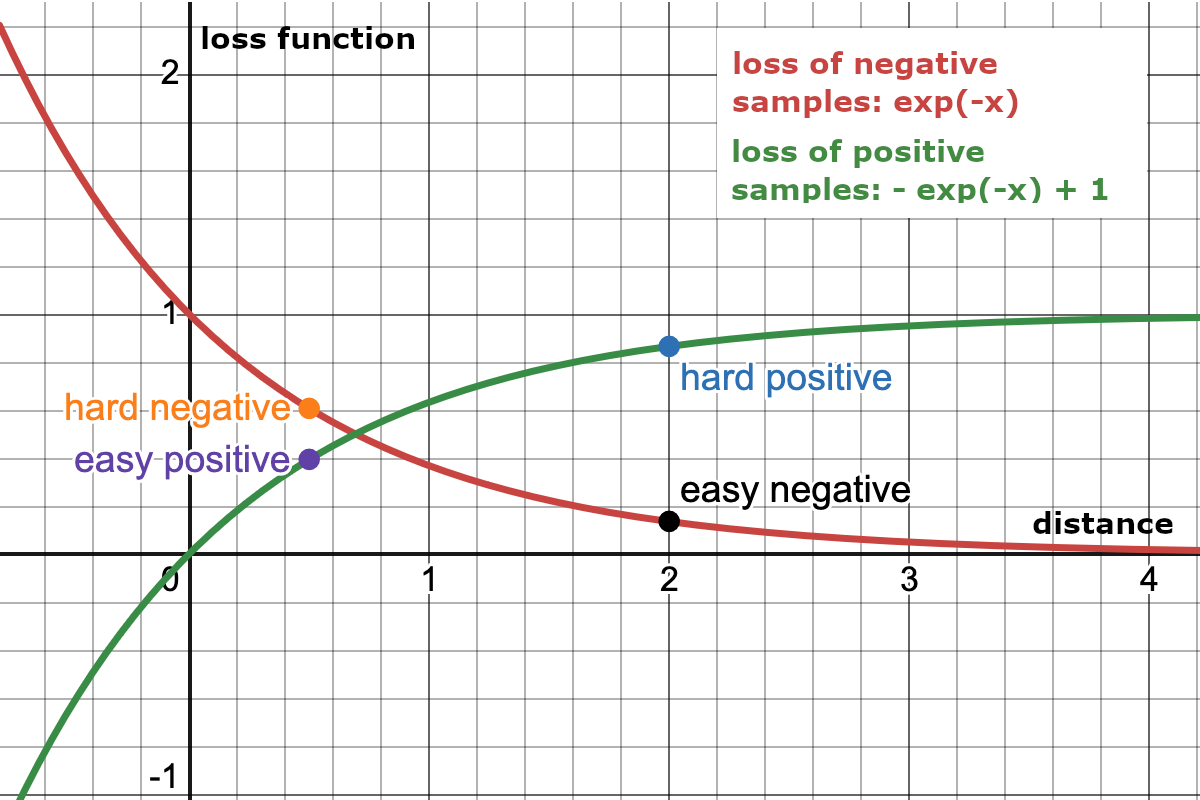
\includegraphics[width=280pt]{images/Hard_easy_samples_dist_effect_loss_desmos_legend.png}
    \caption{The impact of the distance between sample pairs (x-axis) on the loss function (y-axis).
    The red curve represents the loss function for negative samples, 
    whereas the green curve denotes the loss function for positive samples.
    Hard samples have a higher loss value and thus, convey more gradient information than easy samples.
    While distant positive pairs are considered hard, for negative samples, small proximity ones are considered hard.}
    \label{fig:hard_easy_samples_dist_effect_loss}
\end{figure}